\documentclass{beamer}
\usetheme{CVUTFIT}
\usepackage{csquotes}
\usepackage{bibentry}
\usepackage[style=iso-numeric]{biblatex}
\addbibresource{bib-database.bib}
\setbeamertemplate{bibliography item}{\insertbiblabel}

\title[Emulátor konzole NES]{Emulátor konzole Nintendo~Entertainment~System}
\subtitle{Bakalářská práce}
\author[Ondřej Golasowski]{Ondřej Golasowski\texorpdfstring{\\}{}Vedoucí práce: Ing.~Stanislav Jeřábek}
\institute[FIT ČVUT]{Katedra číslicového návrhu, FIT ČVUT}
\date{\today}

\begin{document}
	
\begingroup
\setbeamertemplate{footline}{}
\begin{frame}[noframenumbering]
	\titlepage
\end{frame}
\endgroup

\section{Úvod}
\begin{frame}
	\frametitle{Představení problematiky}
	\begin{definice}[Emulátor]
		Emulátor je software, který umožňuje běh počítačových programů na jiné platformě, než pro kterou byly původně vytvořeny~\normalfont{\cite{Nash1989:sw-emulator}}.
	\end{definice}
	\pause
	Rozdíly oproti simulaci:
	\begin{itemize}
		\item Implementuje se pouze model hardwaru.
		\item Spouští se původní (neupravený) software.
	\end{itemize}
\end{frame}

%\begin{frame}
%	\frametitle{Představení problematiky}
%	Konzole Nintendo Entertainment System:
%	\begin{itemize}
%		\item osmibitový zábavní systém vydaný v~roce 1985,
%		\item procesor Ricoh~2A03 (klon MOS~6502),
%		\item zvukový syntezátor,
%		\item grafický čip Ricoh~2C02,
%		\item distribuce softwaru na kazetách.
%	\end{itemize}
%	\begin{figure}
%		\centering
%		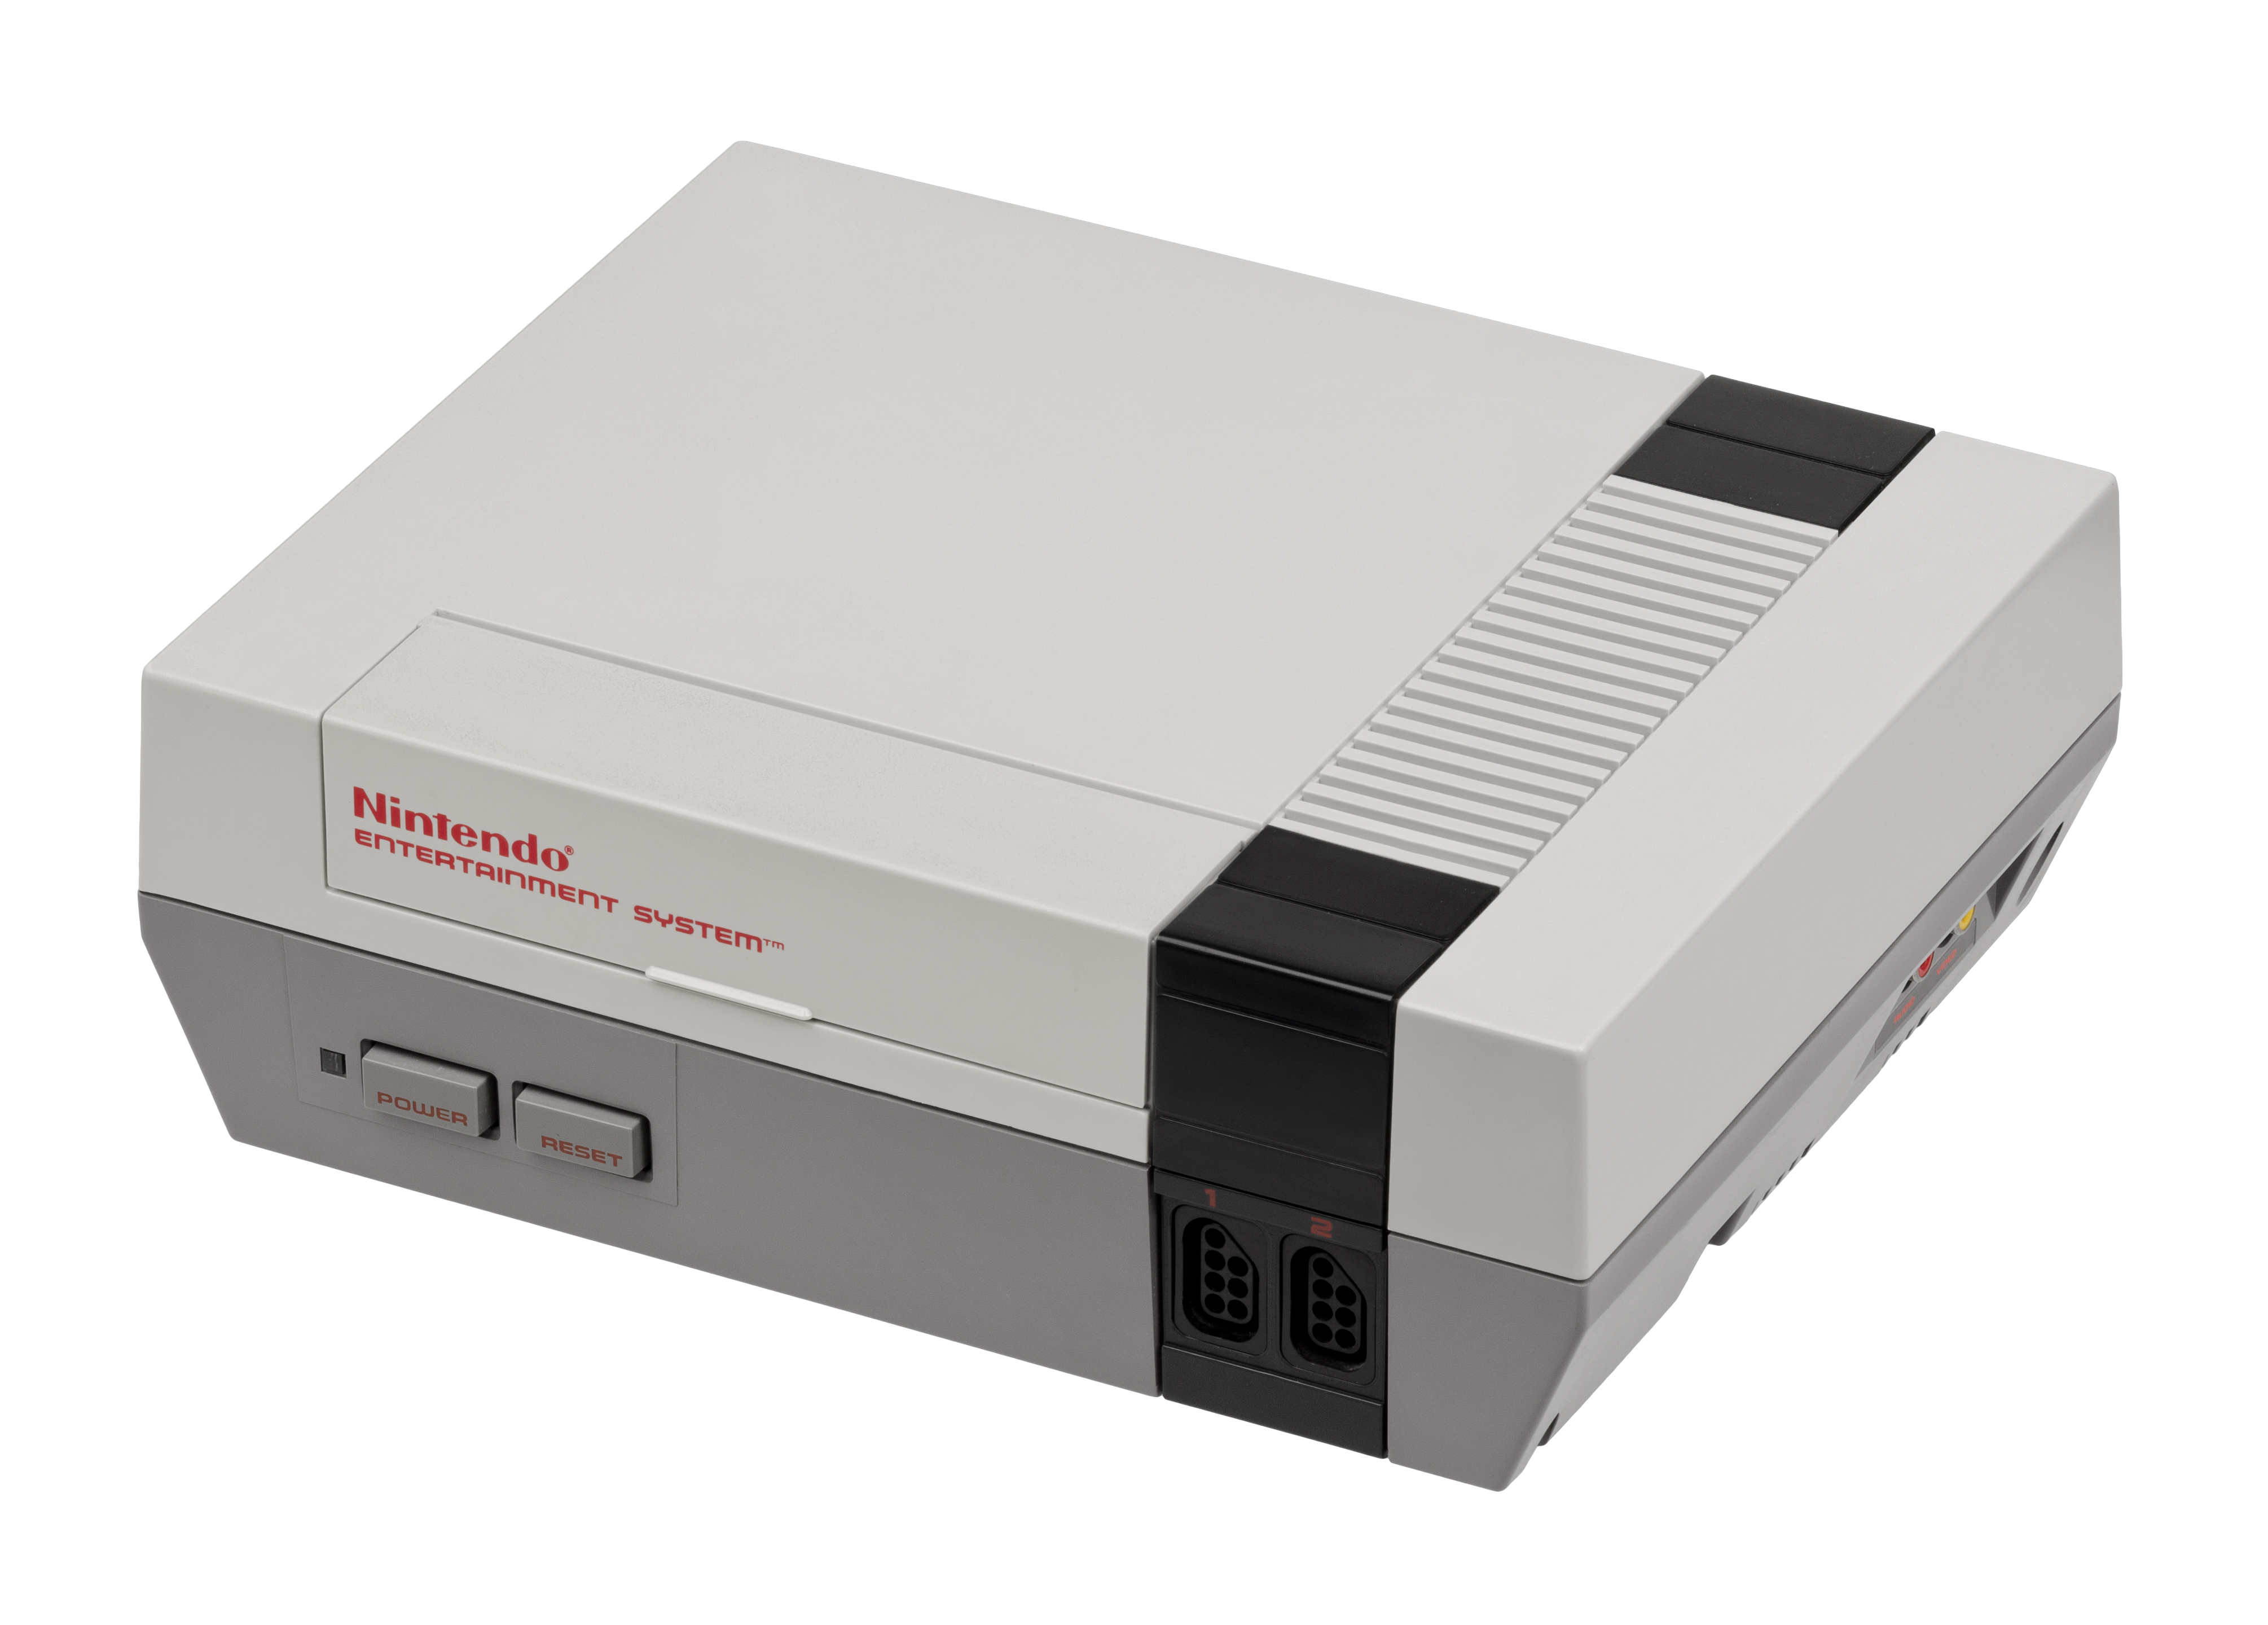
\includegraphics[width=0.3\textwidth]{images/nes.jpg}
%		\caption{Konzole NES (foto \copyright~2016, Evan-Amos)}
%	\end{figure}
%\end{frame}


\begin{frame}
	\frametitle{Motivace a~cíle}
	Motivace:
	\begin{itemize}
		\item Emulátor jako učební pomůcka.
		\begin{itemize}
			\item Zobrazení vnitřních stavů systému.
		\end{itemize}
		\item Vývoj emulátoru jako způsob sebevzdělávání.
		\begin{itemize}
			\item Vhled do zpracování instrukcí, obsluhy přerušení, zobrazování grafiky, syntézy zvuku\dots
		\end{itemize}
	\end{itemize}
	\pause
	Cíle:
	\begin{enumerate}
		\item Vytvořit emulátor atraktivního systému:
		\begin{itemize}
			\item Herní konzole Nintendo Entertainment System (NES).
		\end{itemize}
		\item Zjednodušit vývoj emulátoru ostatním:
		\begin{itemize}
			\item Vytvoření emulační platformy.
		\end{itemize}
	\end{enumerate}
\end{frame}

%\section{Praktická část}
%\begin{frame}
%	\frametitle{Praktická část}
%	Probíhala v~několika fázích:
%	\begin{enumerate}
%		\item Návrh projektu --- technologie.
%		\item Vytvoření modelu emulovaných komponent.
%		\item Vytvoření emulační platformy.
%		\item Integrace emulovaných komponent.
%	\end{enumerate}
%\end{frame}

\begin{frame}
	\frametitle{Vlastnosti řešení}
	\begin{figure}
		\centering
		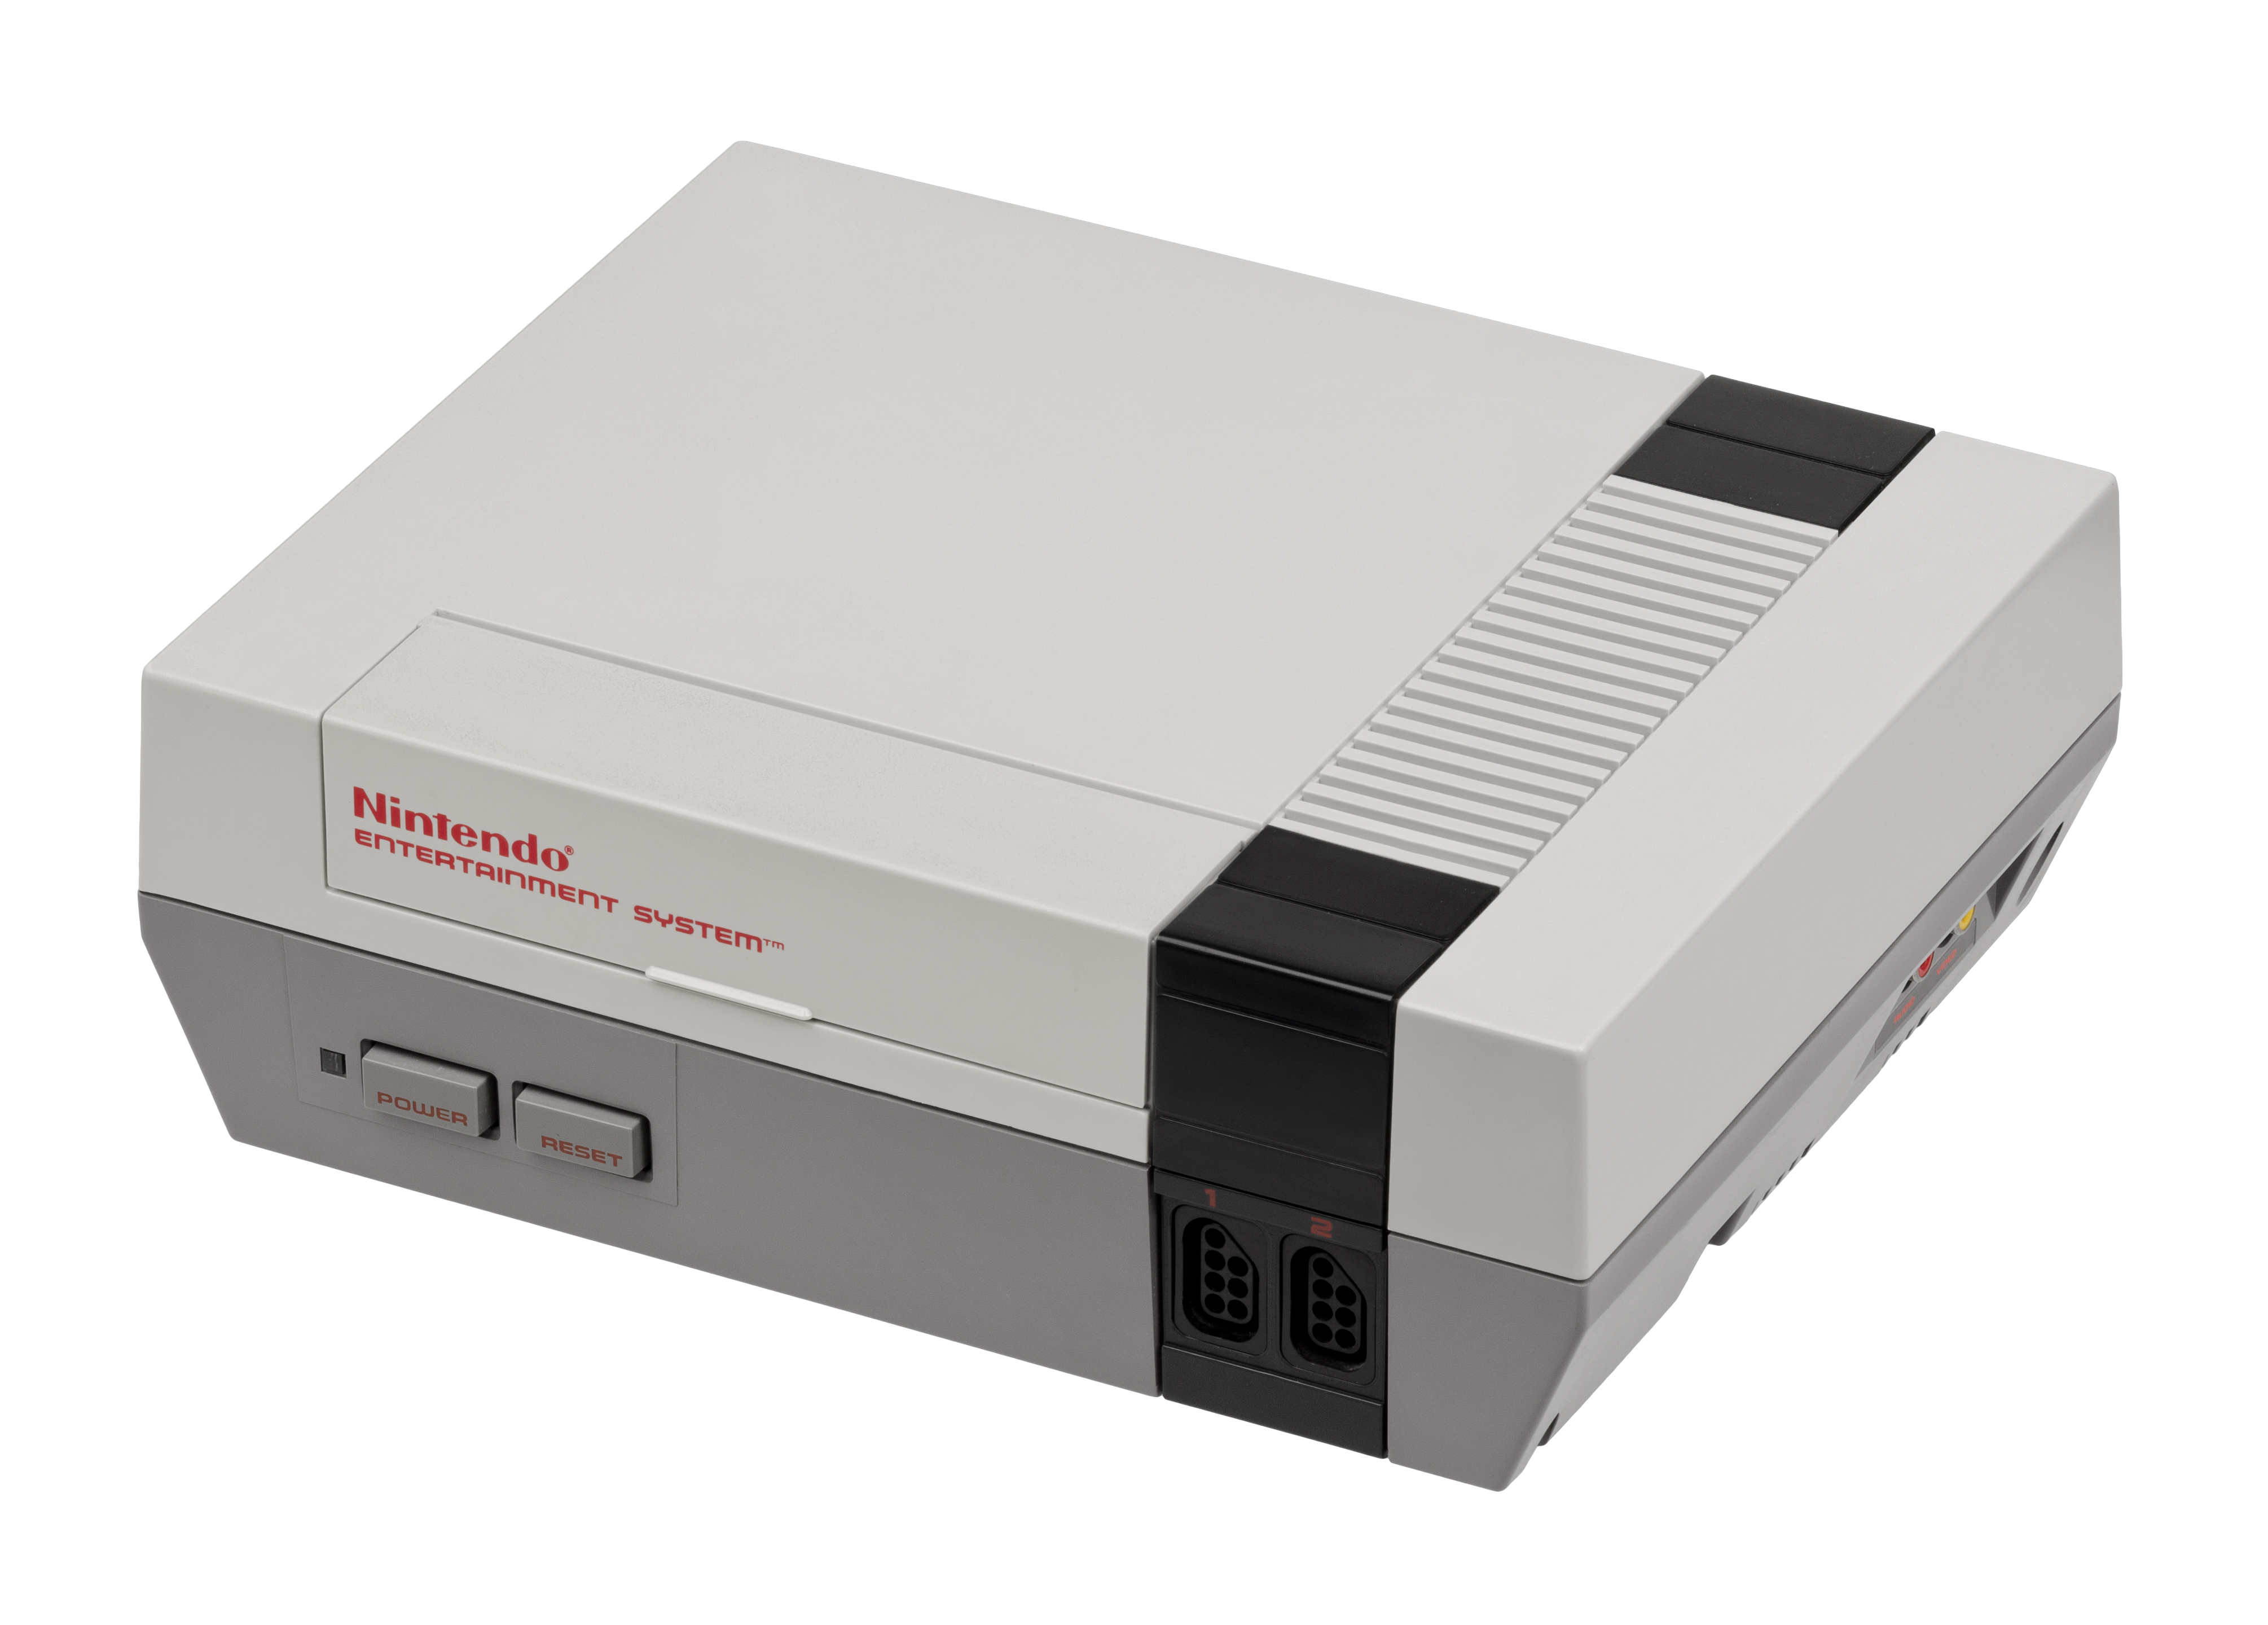
\includegraphics[width=0.25\textwidth]{images/nes.jpg}
		\caption{Konzole NES (foto \copyright~2016, Evan-Amos).}
	\end{figure}
	Emulátor NES:
	\begin{itemize}
		\item Implementovány veškeré komponenty NES.
		\pause
		\item Přehledné zobrazení vnitřních stavů v~emulátoru.
		\pause
		\item Možnost spouštět jednoduché i~složitější hry.
		\pause
		\item Srozumitelný kód, podrobná dokumentace a~manuály.
		\pause
		\item Integrováno do vlastní emulační platformy.
	\end{itemize}
\end{frame}

\begin{frame}
	\frametitle{Vlastnosti řešení}
	\begin{figure}
		\centering
		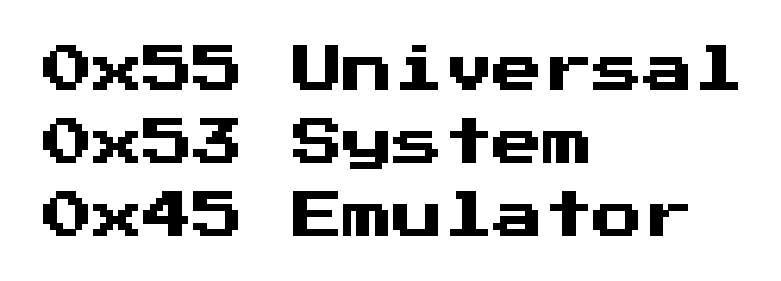
\includegraphics[width=0.5\textwidth]{images/logo-full-path.pdf}
	\end{figure}
	Univerzální emulační platforma
	\begin{itemize}
		\item Jednotný způsob tvorby komponent a~systémů.
		\pause
		\item Libovolná úroveň abstrakce --- od hradel až po čip.
		\pause
		\item Připravena snadná tvorba GUI a~zvukového výstupu.
		\pause
		\item Multiplatformní --- GNU/Linux, macOS, Windows\dots
		\pause
		\item Moderní toolchain: C++20, CMake, CTest, Sphinx.
		\pause
		\item Snadno přístupné: open-source na GitHubu.
		\begin{itemize}
			\item Dostupné na~\url{https://golas.me/use/}
			\item Dokumentace na~\url{https://golas.me/usedocs/}
		\end{itemize}
	\end{itemize}
\end{frame}

\begin{frame}
	\frametitle{Ukázka}
	\begin{figure}
		\centering
		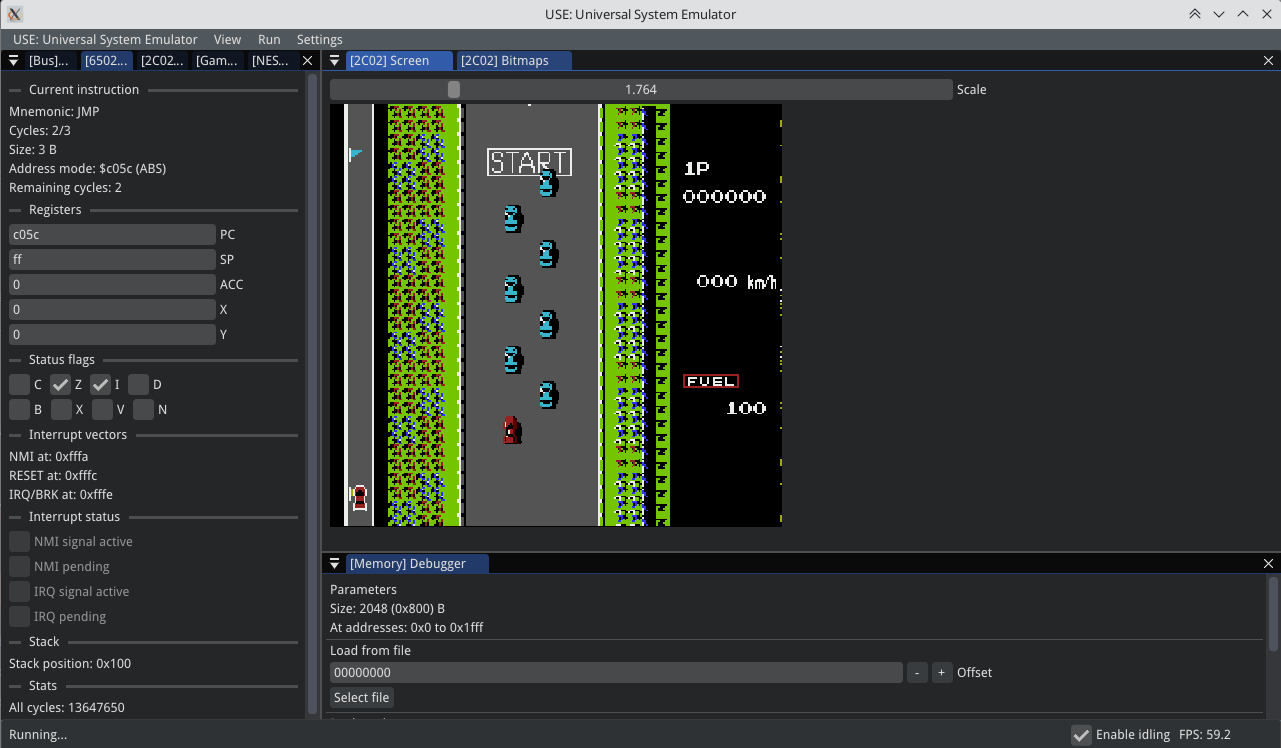
\includegraphics[width=1\textwidth]{images/ss_nes_game_loaded.png}
		\caption{\small Hra \enquote{Road Fighters} spuštěná na emulátoru.}
	\end{figure}
\end{frame}

\begin{frame}
	\frametitle{Shrnutí}
	Během 2~let vzniklo následující:
	\begin{itemize}
		\item Přehledný emulátor NES.
		\pause
		\item Podrobná webová dokumentace.
		\pause
		\item Přehled celého procesu vývoje v~textu práce.
		\pause
		\item Další projekty:
		\begin{itemize}
			\item Pomůcka pro vývojáře emulátorů.
			\item Přídavek do grafické knihovny.
			\item Automatické testy pro MOS~6502.
		\end{itemize}
		\pause
	\end{itemize}
	Potenciální navazující práce:
	\begin{itemize}
		\item Rozšíření emulace NES.
		\pause
		\item Využití v~záverečných pracích (maturitní, bakalářské).
		\pause
		\item Podpora komponent ve Verilogu:
		\begin{itemize}
			\item Simulace RISC-V mikroarchitektur.
		\end{itemize}
	\end{itemize}
\end{frame}

\begin{frame}
	\huge{Děkuji za pozornost.}	
\end{frame}

\begin{frame}
	\frametitle{Reference}
	\printbibliography
\end{frame}

\appendix

\begin{frame}
	\frametitle{Otázky oponenta práce}
	\begin{itemize}
		\item Otázka 1.
		\pause
		\item Otázka 2.
		\pause
		\item Otázka 3.
	\end{itemize}
\end{frame}

\begin{frame}
	\frametitle{Hardware konzole NES}
	\begin{itemize}
		\item Procesor Ricoh 2A03 (klon MOS 6502).
		\item Zvukový syntezátor.
		\begin{itemize}
			\item 4 různé kanály.
		\end{itemize}
		\item Grafický čip Ricoh 2C02.
		\begin{itemize}
			\item Přímo generuje NTSC.
			\item Hardware podpora sprajtů.
		\end{itemize}
		\item Kazety pro distribuci softwaru.
		\begin{itemize}
			\item Obsahují sofistikované mapovací obvody.
		\end{itemize}
		\item Periferie (herní ovladače).	
	\end{itemize}
\end{frame}

\begin{frame}
	\frametitle{Diagram tříd platformy}
	\begin{figure}
		\centering
		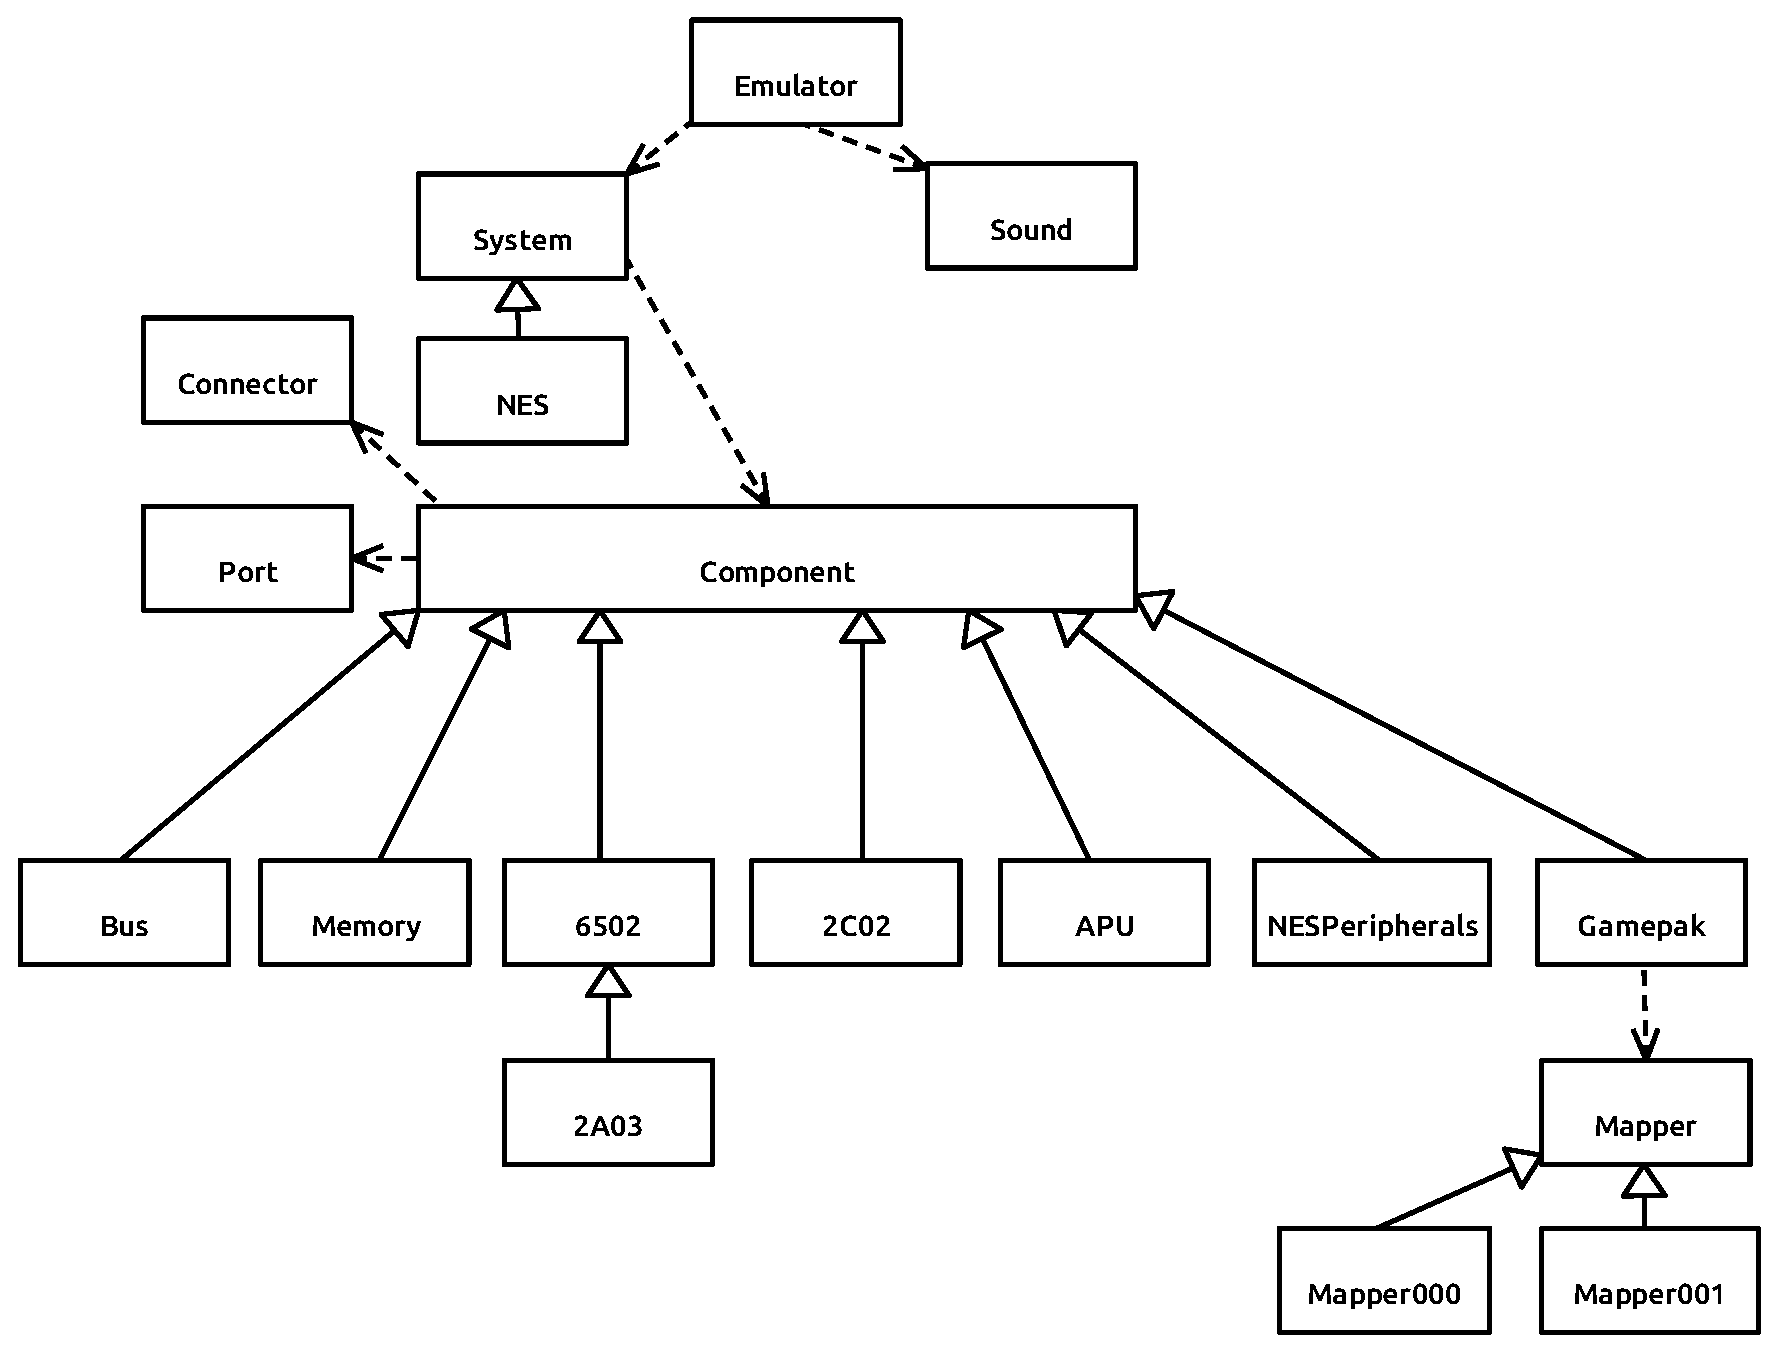
\includegraphics[width=0.8\textwidth]{images/navrh_prehled.pdf}
		\caption{\normalsize Přehledový diagram tříd.}
	\end{figure}
\end{frame}
	
\begin{frame}
	\frametitle{Webová dokumentace}
	\begin{figure}
		\centering
		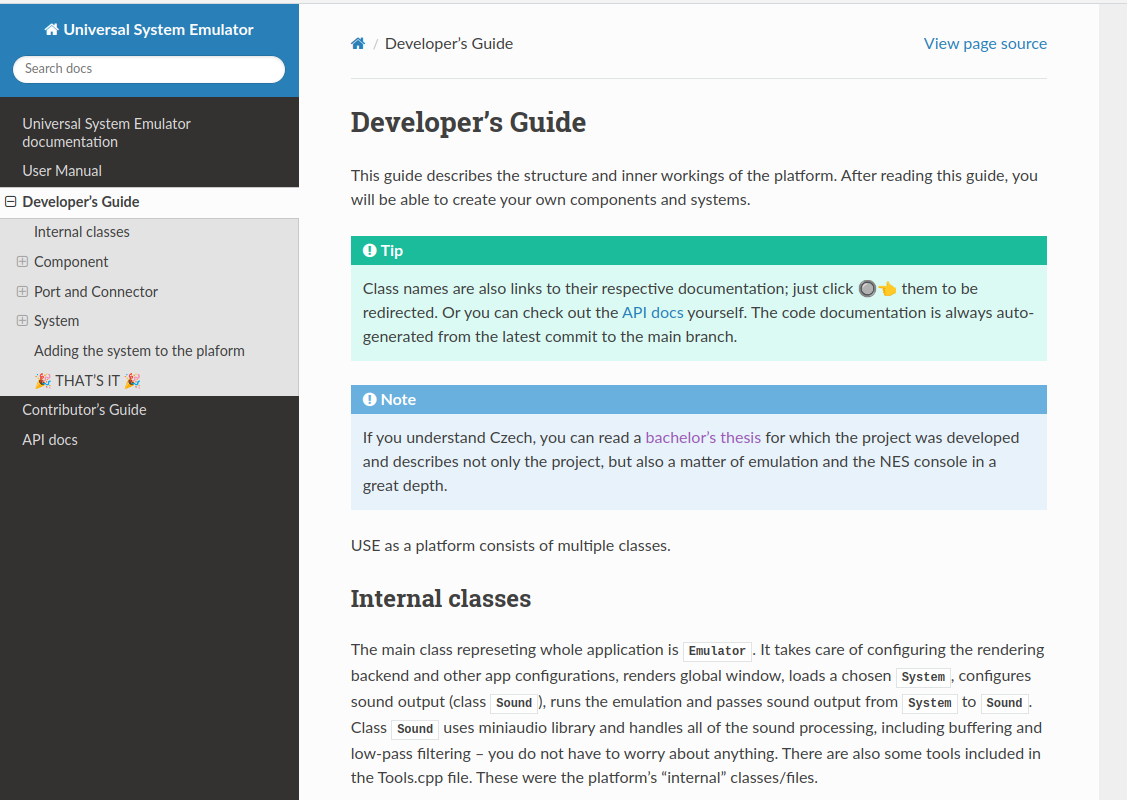
\includegraphics[width=0.8\textwidth]{images/docs.png}
		\caption{\normalsize Webová dokumentace k~projektu.}
	\end{figure}
\end{frame}
	
\end{document}